% =============================================================================
% PALACE SIGNAL-FLOW / TECHNICAL DIAGRAM TEMPLATE  (TikZ + standalone)
% -----------------------------------------------------------------------------
% Copy this file, rename it, edit the tikzpicture body. The style block below
% gives you the four DSP signal-flow primitives:
%   adder   -- summing junction (circle with +)
%   gainf   -- gain, triangle pointing RIGHT  (feed-forward)
%   gainb   -- gain, triangle pointing LEFT   (feed-back)
%   delay   -- unit delay block (z^{-1})
%   tap     -- branch/junction dot
%
% RENDER (see render.sh, or run by hand):
%   pdflatex <file>.tex
%   dvisvgm --pdf --no-fonts <file>.pdf -o <file>.svg   # text -> vector outlines
%   # ...or keep text editable as text (embeds the font):
%   dvisvgm --pdf --font-format=woff <file>.pdf -o <file>.svg
% The .svg opens and edits in Inkscape / Affinity Designer / Figma.
% =============================================================================
\documentclass[border=6pt]{standalone}
\usepackage{amsmath}
\usepackage{tikz}
\usetikzlibrary{shapes.geometric, arrows.meta, positioning, calc}

\tikzset{
  >={Stealth[length=2.4mm]},
  wire/.style ={line width=0.7pt},
  adder/.style={circle, draw, line width=0.7pt, minimum size=6mm, inner sep=0pt},
  gainf/.style={isosceles triangle, draw, line width=0.7pt,
                isosceles triangle apex angle=55, minimum width=9mm, inner sep=2pt},
  gainb/.style={gainf, shape border rotate=180},
  delay/.style={rectangle, draw, line width=0.7pt, minimum size=8mm, inner sep=2pt},
  tap/.style  ={circle, fill, minimum size=3.4pt, inner sep=0pt},
}

\begin{document}
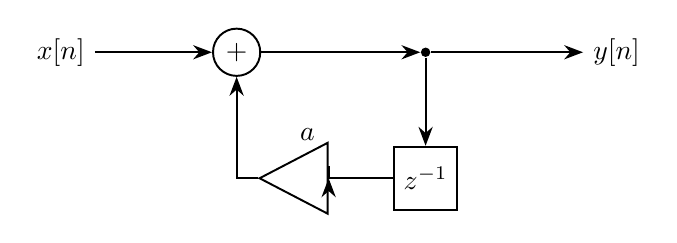
\begin{tikzpicture}
  % --- minimal example: one-pole feedback (leaky integrator) ----------------
  \node[adder] (s)  at (0,0)   {$+$};
  \node[tap]   (t)  at (2.4,0) {};
  \node[delay] (d)  at (2.4,-1.6) {$z^{-1}$};
  \node[gainb] (g)  at (0.9,-1.6) {}; \node at (0.9,-1.05) {$a$};

  \draw[wire,->] (-1.8,0) node[left]{$x[n]$} -- (s);
  \draw[wire,->] (s) -- (t);
  \draw[wire,->] (t) -- (4.4,0) node[right]{$y[n]$};
  \draw[wire,->] (t) -- (d);
  \draw[wire,->] (d) -| (g.east);           % delay output into feed-back gain
  \draw[wire,->] (g.west) -| (s.south);     % gain back into summing node
\end{tikzpicture}
\end{document}
